%%%
%
% $Autor: Wings $
% $Datum: 2021-05-14 $
% $Pfad: GitLab/MLEdgeComputer $
% $Dateiname: HeartRate.tex
% $Version: 4620 $
%
% !TeX spellcheck = de_DE/GB
% !TeX program = pdflatex
% !BIB program = biber/bibtex
% !TeX encoding = utf8
%
%%%
\chapter{Heart Rate Sensor}

\section{The Heartbeat}
{
    \subsection{Introduction}
    
    The heartbeat, also known as pulse or heart rhythm, is a central element of the human circulatory system. The heart is a muscular hollow organ, approximately the size of a fist, located in the thorax between the lungs. It consists of four chambers: the two atria and the two ventricles. This anatomy allows the heart to pump blood efficiently throughout the body, supplying tissues and organs with oxygen and nutrients while removing waste products. \cite{Gesenberg:2017}
    
    \subsection{Cardiac Cycle}
    
    The heartbeat occurs in a regular cycle known as the cardiac cycle. This cycle consists of two main phases: diastole and systole. During diastole, the heart relaxes and fills with blood from the atria. The atria contract to pump blood into the ventricles; the ventricles then contract to pump blood out of the heart and into the circulatory system. This rhythmic alternation between contraction and relaxation enables efficient blood flow throughout the body. \cite{Gesenberg:2017}
    
    \subsection{Electrical Activity}
    
    The electrical activity of the heart plays a crucial role in controlling the heartbeat. The sinoatrial node, also known as the natural pacemaker of the heart, is located in the right atrium and sends out electrical signals that initiate the contraction of the heart muscle. These electrical impulses spread through specialized conduction pathways within the heart, such as the AV node and the bundle of His, stimulating the synchronized contraction of the entire heart muscle. \cite{Gesenberg:2017}
    
    \subsection{Heart Rate}
    
    Heart rate, measured in beats per minute (\ac{bpm}), varies depending on factors such as age, fitness level, and individual conditions. The average resting heart rate for adults is typically between 60 and 100 beats per minute. A lower heart rate can indicate good heart health and efficient heart function. An elevated heart rate, however, may result from factors such as stress, physical activity, or illness. \cite{Sammito:2021}
    
    Figure \ref{HeartRateFrequencies} shows an example frequency. The x-axis represents time in seconds (s), and the y-axis represents the frequency in \ac{bpm}. The RR interval is the distance between two R peaks in an ECG, from which the \ac{hr} can be mathematically derived:
    
    \Mynote{R peak? RR? ECG? Picture?}
    \[
    \text{HR} \left[\frac{1}{\text{min}}\right] = \frac{60}{\text{RR interval} \left[\text{s}\right]}
    \]
    
    \begin{center}
        \begin{tikzpicture}[scale=6,]
            
            \draw (0.6,0.1) -- (1.8,0.1);
            \draw (0.6,0.1) -- (0.6,0.9);
            \draw [fill=black](0.58,0.9) -- (0.62,0.9) -- (0.6,0.95) -- cycle;
            \draw [fill=black](1.8,0.08) -- (1.8,0.12) -- (1.85,0.1) -- cycle;
            
            \draw[red] (0.6,0.45)--(0.7,0.45);
            \draw[red] (0.7,0.45)--(0.72,0.41);   
            \draw[red] (0.72,0.41)--(0.75,0.47);
            \draw[red] (0.75,0.47)--(0.77,0.43);
            \draw[red] (0.77,0.43)--(0.83,0.55);
            \draw[red] (0.83,0.55)--(0.93,0.35);
            \draw[red] (0.93,0.35)--(0.98,0.45);
            \draw[red] (0.98,0.45)--(1.05,0.45);     
            \draw[red] (1.05,0.45)--(1.065,0.48);
            \draw[red] (1.065,0.48)--(1.08,0.45);
            
            \draw[red] (1.08,0.45)--(1.3,0.45);
            \draw[red] (1.3,0.45)--(1.32,0.41);   
            \draw[red] (1.32,0.41)--(1.35,0.47);
            \draw[red] (1.35,0.47)--(1.37,0.43);
            \draw[red] (1.37,0.43)--(1.43,0.55);
            \draw[red] (1.43,0.55)--(1.53,0.35);
            \draw[red] (1.53,0.35)--(1.58,0.45);
            \draw[red] (1.58,0.45)--(1.65,0.45);     
            \draw[red] (1.65,0.45)--(1.665,0.48);
            \draw[red] (1.665,0.48)--(1.68,0.45);
            \draw[red] (1.68,0.45)--(1.7,0.45);
            
            \node at (0.83,1){Frequency in bpm};
            \node at (1.7,0.05) {Time in s};
            
            \draw (0.83,0.6)--(1.43,0.6);
            \draw (0.83,0.58)--(0.83,0.62);
            \draw (1.43,0.58)--(1.43,0.62);
            
            \node at (1.13,0.65){R-R interval};
            
        \end{tikzpicture}
        
        \captionof{figure}]{Example frequency of a heartbeat}  \label{HeartRateFrequencies}	
    \end{center}
    
    \subsection{Regulation of the Heartbeat}
    
    The heartbeat is regulated by various factors. In addition to the central nervous system, which can increase or decrease the heart rate as needed, hormones like adrenaline and noradrenaline, as well as certain medications, can influence the heartbeat. Emotions such as fear or excitement can also impact the heartbeat by activating the sympathetic nervous system, leading to an increased heart rate. \cite{Gesenberg:2017}
    
    \subsection{Heartbeat Deviations}
    
    Deviations in the heartbeat, such as arrhythmias (irregular heart rhythms), can be caused by various factors, including heart disease, electrolyte imbalances, or medications. An elevated heart rate (tachycardia) or a decreased heart rate (bradycardia) can also indicate medical issues and may require clinical examination and treatment. \cite{Gesenberg:2017}
    
    \Mynote{Sieht man das in den Daten?}
}



\section{Operation of the Heartbeat Sensor}
{	
    The sensor ``GRV Heart Rate 3'' is an optical heart rate sensor that uses photoplethysmography (\ac{ppg}) to measure heart rate. \cite{Gitman:2023}
    
    
    \begin{center}
        \centering
        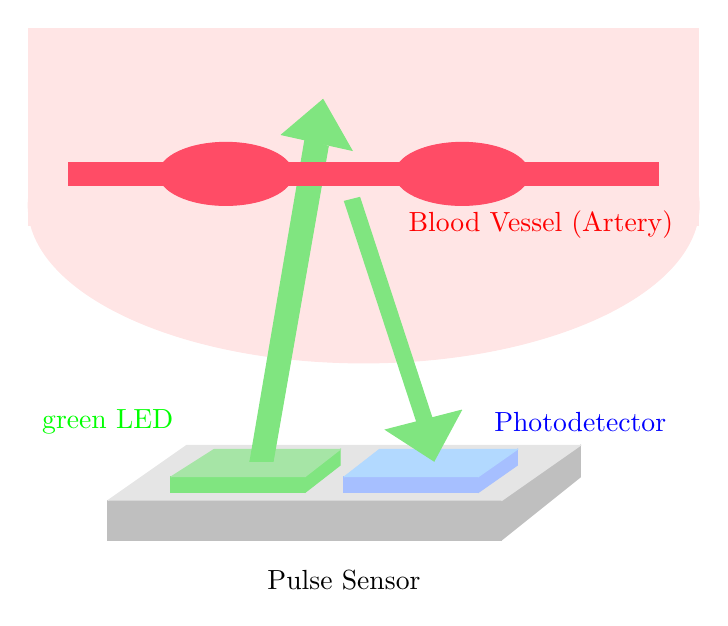
\begin{tikzpicture}
            \draw [fill=lightgray, draw=lightgray] (-2,0) rectangle (3,0.5);
            \draw [fill=lightgray, draw=lightgray] (3,0)--(4,0.8)--(4,1.2)--(3,0.5);
            \definecolor{verylightgray}{gray}{0.9};
            \draw [fill=verylightgray, draw=verylightgray] (-2,0.5)--(-1,1.2)--(4,1.2)--(3,0.5);
            
            \definecolor{lightgreen}{rgb}{0.5, 0.9, 0.5};
            \draw [fill=lightgreen, draw=lightgreen] (-1.2,0.6) rectangle (0.5,0.8);
            \draw [fill=lightgreen, draw=lightgreen] (0.5,0.8)--(0.95,1.15)--(0.95,0.95)--(0.5,0.6);
            
            \definecolor{hautfarbe}{rgb}{1, 0.9, 0.9};
            \draw [fill=hautfarbe, draw=hautfarbe] (-3,4) rectangle (5.5,6.5);
            \draw [fill=hautfarbe, draw=hautfarbe] (1.25,4.25) ellipse (4.26cm and 2cm);
            
            \definecolor{verylightgreen}{rgb}{0.65, 0.9, 0.65};
            \draw [fill=verylightgreen, draw=verylightgreen] (-1.2,0.8)--(-0.65,1.15)--(0.95,1.15)--(0.5,0.8);
            
            \definecolor{lightblue}{rgb}{0.65, 0.75, 1};
            \draw [fill=lightblue, draw=lightblue] (1,0.6) rectangle (2.7,0.8);
            \draw [fill=lightblue, draw=lightblue] (2.7,0.8)--(3.2,1.15)--(3.2,0.95)--(2.7,0.6);
            
            \definecolor{verylightblue}{rgb}{0.7, 0.85, 1};
            \draw [fill=verylightblue, draw=verylightblue] (1,0.8)--(1.45,1.15)--(3.2,1.15)--(2.7,0.8);
            
            \draw [fill=lightgreen, draw=lightgreen] (-0.2,1)--(0.1,1)--(0.8,5)--(0.5,5.1);
            \draw [fill=lightgreen, draw=lightgreen] (0.2,5.15)--(1.1,4.95)--(0.73,5.6);
            \draw [fill=lightgreen, draw=lightgreen] (1,4.3)--(1.2,4.35)--(2.2,1.3)--(2,1.25);
            \draw [fill=lightgreen, draw=lightgreen] (2.15,1)--(1.53,1.4)--(2.5,1.65);
            
            \definecolor{lightred}{rgb}{1, 0.3, 0.4};
            \draw [fill=lightred, draw=lightred] (0,4.5) rectangle (2,4.8);
            \draw [fill=lightred, draw=lightred](-0.5,4.65) ellipse (0.85cm and 0.4cm);
            \draw [fill=lightred, draw=lightred](2.5,4.65) ellipse (0.85cm and 0.4cm);
            \draw [fill=lightred, draw=lightred] (3,4.5) rectangle (5,4.8);
            \draw [fill=lightred, draw=lightred] (-0.5,4.5) rectangle (-2.5,4.8);
            
            \node[green] at (-2,1.5){green LED};
            \node[blue] at (4,1.5){Photodetector};
            \node at (1,-0.5){Pulse Sensor};
            \node[red] at (3.5,4){Blood Vessel (Artery)};	
            
        \end{tikzpicture}
        
        \captionof{figure}{Photoplethysmography}\label{fig:Photoplethysmography}	
    \end{center}
    
    \begin{itemize}
        \item \textbf{Light Source and Photodetector:} The sensor consists of \ac{led}s (usually green light) and a photodetector. The LEDs emit light into the skin.
        \item \textbf{Measurement of Light Reflection:} The light is directed into the skin and is partially absorbed by the blood vessels. The photodetector measures the amount of reflected light.
        \item \textbf{Detection of Blood Flow Changes:} With each heartbeat, the amount of reflected light changes due to the varying blood flow in the vessels. These changes are detected by the photodetector.
        \item \textbf{Calculation of Heart Rate:} The changes in light reflection caused by the pulse are used to calculate the heart rate.
    \end{itemize}
    
    \Mynote{more explanations}
    
    The functional principle of the sensor is shown schematically in Figure \ref{fig:Photoplethysmography}.
    
    \subsection{The Photodetector}
    
    
    The photodetector utilizes the photoelectric effect, a phenomenon where electrons are emitted from a material (usually a metal) when it is exposed to light. \cite{Traenkler:2014}.
    Figure \ref{fig:PhotoelectricEffect} illustrates this phenomenon.
    
    
    \begin{figure}[h]
        \centering
        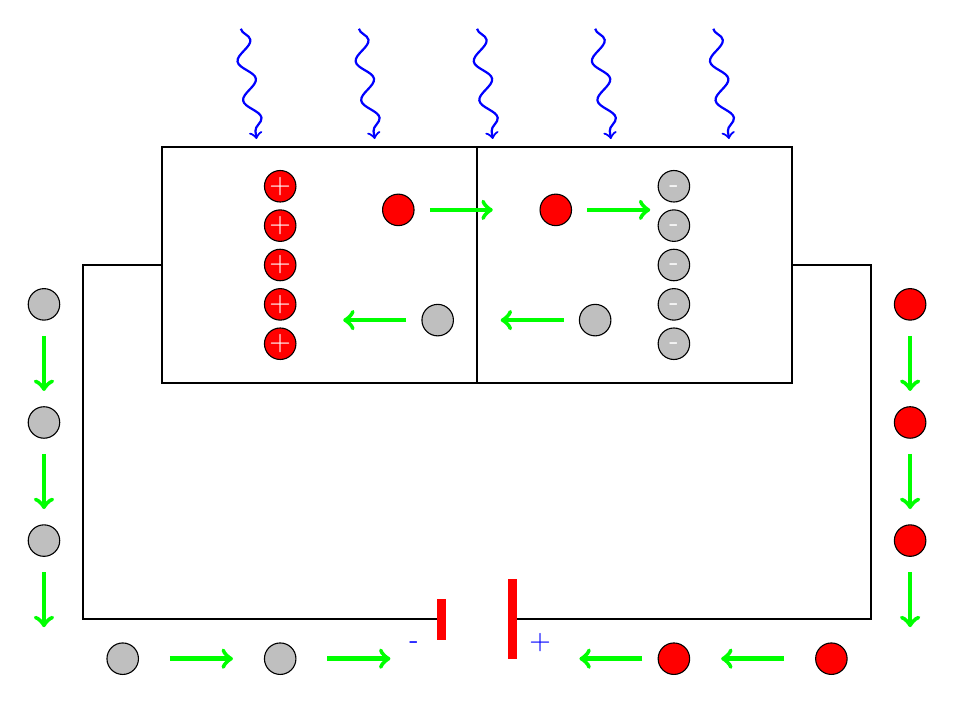
\begin{tikzpicture}
            \draw [thick] (0,0)rectangle(8,3);
            \draw (4,3)--(4,0);
            \draw [thick] (0,1.5)--(-1,1.5)--(-1,-3)--(3.5,-3);
            \draw [thick] (8,1.5)--(9,1.5)--(9,-3)--(4.5,-3);
            \draw [fill=red, draw=red] (3.5,-3.25) rectangle (3.6,-2.75);
            \draw [fill=red, draw=red] (4.5,-3.5) rectangle (4.4,-2.5);
            \node [thick,blue] at(3.2,-3.3){-};
            \node [thick,blue] at(4.8,-3.3){+};
            
            \draw[fill=lightgray] (6.5,0.5) circle (0.2cm);
            \draw[fill=lightgray] (6.5,1) circle (0.2cm);
            \draw[fill=lightgray] (6.5,1.5) circle (0.2cm);
            \draw[fill=lightgray] (6.5,2) circle (0.2cm);
            \draw[fill=lightgray] (6.5,2.5) circle (0.2cm);
            
            \draw[fill=red] (1.5,0.5) circle (0.2cm);
            \draw[fill=red] (1.5,1) circle (0.2cm);
            \draw[fill=red] (1.5,1.5) circle (0.2cm);
            \draw[fill=red] (1.5,2) circle (0.2cm);
            \draw[fill=red] (1.5,2.5) circle (0.2cm);
            
            \draw[fill=lightgray] (5.5,0.8) circle (0.2cm);
            \draw[fill=lightgray] (3.5,0.8) circle (0.2cm);
            
            \draw[->,ultra thick,green](5.1,0.8) -- (4.3,0.8);
            \draw[->,ultra thick,green](3.1,0.8) -- (2.3,0.8);
            
            \draw[fill=red] (3,2.2) circle (0.2cm);
            \draw[fill=red] (5,2.2) circle (0.2cm);
            
            \draw[->,ultra thick,green](3.4,2.2) -- (4.2,2.2);
            \draw[->,ultra thick,green](5.4,2.2) -- (6.2,2.2);
            
            \draw[fill=lightgray] (-1.5,-2) circle (0.2cm);
            \draw[fill=lightgray] (-1.5,1) circle (0.2cm);
            \draw[fill=lightgray] (-1.5,-0.5) circle (0.2cm);
            \draw[fill=lightgray] (-0.5,-3.5) circle (0.2cm);
            \draw[fill=lightgray] (1.5,-3.5) circle (0.2cm);
            
            \draw[->,ultra thick,green](-1.5,0.6) -- (-1.5,-0.1);
            \draw[->,ultra thick,green](-1.5,-0.9) -- (-1.5,-1.6);
            \draw[->,ultra thick,green](-1.5,-2.4) -- (-1.5,-3.1);
            \draw[->,ultra thick,green](0.1,-3.5) -- (0.9,-3.5);
            \draw[->,ultra thick,green](2.1,-3.5) -- (2.9,-3.5);
            
            \draw[fill=red] (9.5,-2) circle (0.2cm);
            \draw[fill=red] (9.5,1) circle (0.2cm);
            \draw[fill=red] (9.5,-0.5) circle (0.2cm);
            \draw[fill=red] (8.5,-3.5) circle (0.2cm);
            \draw[fill=red] (6.5,-3.5) circle (0.2cm);
            
            \draw[->,ultra thick,green](9.5,0.6) -- (9.5,-0.1);
            \draw[->,ultra thick,green](9.5,-0.9) -- (9.5,-1.6);
            \draw[->,ultra thick,green](9.5,-2.4) -- (9.5,-3.1);
            \draw[->,ultra thick,green](7.9,-3.5) -- (7.1,-3.5);
            \draw[->,ultra thick,green](6.1,-3.5) -- (5.3,-3.5);
            
            \draw[thick,blue,->, decorate, decoration={snake, amplitude=1mm, segment length=5mm}] (1,4.5) -- (1.2,3.1);
            \draw[thick,blue,->, decorate, decoration={snake, amplitude=1mm, segment length=5mm}] (2.5,4.5) -- (2.7,3.1);
            \draw[thick,blue,->, decorate, decoration={snake, amplitude=1mm, segment length=5mm}] (4,4.5) -- (4.2,3.1);
            \draw[thick,blue,->, decorate, decoration={snake, amplitude=1mm, segment length=5mm}] (5.5,4.5) -- (5.7,3.1);
            \draw[thick,blue,->, decorate, decoration={snake, amplitude=1mm, segment length=5mm}] (7,4.5) -- (7.2,3.1);
            
            \node [thick,white] at (6.5,0.5) {-};
            \node [thick,white] at (6.5,1) {-};
            \node [thick,white] at (6.5,1.5) {-};
            \node [thick,white] at (6.5,2) {-};
            \node [thick,white] at (6.5,2.5) {-};
            
            \node [thick,white] at (1.5,0.5) {+};
            \node [thick,white] at (1.5,1) {+};
            \node [thick,white] at (1.5,1.5) {+};
            \node [thick,white] at (1.5,2) {+};
            \node [thick,white] at (1.5,2.5) {+};
            
        \end{tikzpicture}
        
        \caption{The Photoelectric Effect}
        \label{fig:PhotoelectricEffect}	
    \end{figure}
        
	\subsubsection{Output of the Photodetector}

The photodetector generates a voltage that is measured over time. This voltage varies periodically, depending on the amount of reflected light, which is influenced by changes in blood volume caused by the heartbeat.

Therefore, the variation in the photodetector’s voltage is directly correlated with the frequency of the heartbeat. \cite{Traenkler:2014}.


\subsection{Voltage Data Processing}

The sensor ``GRV Heart Rate 3'' outputs analog voltage values ranging from 0 to 3.3 volts. These voltages are captured by the Arduino through an analog input. The Arduino uses its built-in \ac{adc} to convert these analog voltages into digital values. This process is illustrated in Figure \ref{fig:StructureSensor}.

The Arduino’s \ac{adc} has a resolution of 10 bits, meaning it divides the voltage range from 0 to 3.3 volts into 1024 steps. Thus, a voltage of 0 volts is represented as a digital value of 0, and a voltage of 3.3 volts is represented as a digital value of 1023. The voltage values between these two extremes are proportionally converted into corresponding digital values. \cite{Parthier:2016} \Mynote{really proportional?}

This conversion allows the Arduino to process the analog voltages output by the sensor as easily manageable digital values. These digital values are then used in the code to calculate the heart rate by counting the number of peaks in the voltage data over a certain period and converting this into beats per minute.\Mynote{accuracy?}

\bigskip

\begin{center}
    \hspace*{-2.5cm} % Shifts the content to the left
    \begin{adjustbox}{valign=t}
        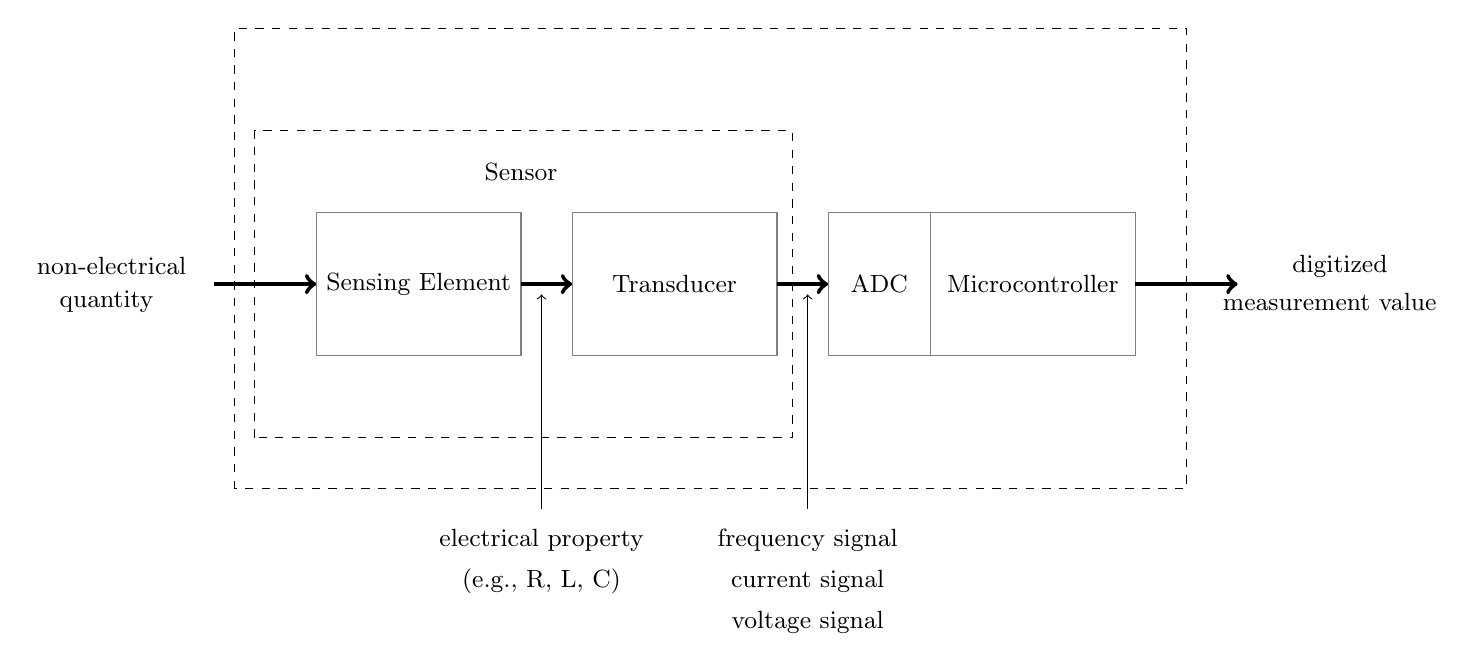
\begin{tikzpicture}[scale=1.3]
            \draw[->,ultra thick](0,0)--(1,0);
            \draw[gray] (1,-0.7) rectangle (3,0.7);
            \draw[->,ultra thick](3,0)--(3.5,0);
            \draw[gray] (3.5,-0.7) rectangle (5.5,0.7);
            \draw[->,ultra thick](5.5,0)--(6,0);
            \draw[gray] (6,-0.7) rectangle (9,0.7);
            \draw[gray] (7,-0.7)--(7,0.7);
            \draw[->,ultra thick](9,0)--(10,0);
            \draw[dashed](0.2,-2)rectangle(9.5,2.5);
            \draw[dashed](0.4,-1.5)rectangle(5.65,1.5);
            
            \draw[<-](3.2,-0.1)--(3.2,-2.2);
            \draw[<-](5.8,-0.1)--(5.8,-2.2);
            
            \node at (3.2,-2.5){\small electrical property};
            \node at (3.2,-2.9){\small (e.g., R, L, C)};
            
            \node at (5.8,-2.5){\small frequency signal};
            \node at (5.8,-2.9){\small current signal};
            \node at (5.8,-3.3){\small voltage signal};
            
            \node at (3,1.1){\small Sensor};
            \node at (2,0){\small Sensing Element};
            \node at (4.5,0){\small Transducer};
            \node at (6.5,0){\small ADC};
            \node at (8,0){\small Microcontroller};
            \node at (-1,0.175){\small non-electrical};
            \node at (-1.05,-0.175){\small quantity};
            
            \node at (11,0.175){\small digitized};
            \node at (10.9,-0.175){\small measurement value};
        \end{tikzpicture}
        
    \end{adjustbox}
    \captionof{figure}{Structure of a Sensor}\label{fig:StructureSensor}\Mynote{smaller}
\end{center}


\subsection{Drift and Measurement Inaccuracies}

Drift can play a significant role in heartbeat sensors. Drift refers to the gradual change in sensor measurements over time, which is not due to actual changes in the measured parameter. In the context of a heartbeat sensor, various types of drift can occur.

A heartbeat sensor converts physiological properties, such as changes in blood flow, into electrical signals for analysis. However, it is possible that the readings fluctuate even though the heart rate remains constant. This unwanted variation in readings is referred to as drift. \cite{Traenkler:2014}. Drift is time-dependent and occurs due to aging processes and inherent inaccuracies of the sensor. In the worst case, drift can lead to the sensor's functional failure.\Mynote{Algorithms? Values?}

\begin{itemize}[label={}]
    
    \item \textbf{Electronic Drift} refers to changes in the electronics of the sensor or the Arduino board itself. Electronic components can change their properties over time due to temperature fluctuations, aging, or other factors, leading to drift in the output values.
    \item \textbf{Optical Drift} occurs in heartbeat sensors that operate based on photoplethysmography (PPG) by measuring the light absorption through the blood. Changes in optical components, such as LEDs or photodetectors, can cause drift, for example, due to contamination, aging of the \ac{led}s, or changes in tissue permeability.
    \item \textbf{Mechanical Drift} can be caused by mechanical changes or shifts of the sensor on the skin. Poor or shifting placement of the sensor can affect the accuracy of the measurements.
    \item \textbf{Calibration Drift} occurs in heartbeat sensors that require regular calibration to ensure accurate measurements. Without regular calibration, the sensor can begin to drift and provide inaccurate readings.
\end{itemize}

Several measures can be taken to minimize the effects of drift:

\begin{itemize}[label={}]
    
    \item \textbf{Regular Calibration}: If the sensor requires calibration, it should be performed regularly to ensure the measurements remain accurate.
    \item \textbf{Continuous Monitoring}: Continuous monitoring of output values and comparison with known reference values (e.g., comparison with a clinically validated device) can help detect and correct drift.
    \item \textbf{Sensor Placement}: Consistent and stable placement of the sensor on the body can minimize mechanical drift. Ideally, the sensor should be attached to an area with minimal movement, such as the earlobe.
    \item \textbf{Environmental Control}: Controlling the temperature and environmental conditions can reduce electronic drift.
\end{itemize}

\Mynote{How to do? Where?}

By considering these measures, the accuracy and reliability of heart rate measurements using the heartbeat sensor can be improved. \cite{Traenkler:2014}. \Mynote{How?}
}



\section{Heart Rate Sensor with Grove Interface and Ear Clip}

The GRV Heart Rate 3 sensor is designed to measure heart rate using infrared light. It detects pulse waves in the bloodstream through an ear-mounted clip (see figure \ref{fig:Herzschlagsensor}), providing continuous heart rate data. This type of measurement is commonly used \Mynote{citations?!} in health monitoring systems and fitness devices.
\cite{Seeed:2024}

\subsection{Key Technical Specifications}

Along the data sheet, see \cite{Seeed:2024}, the sensor has the folloing specifications:

\begin{itemize}
  \item \textbf{Measurement Principle}: Optical pulse detection using infrared light
  \item \textbf{Power Supply}: 3.0V (min), 5.0V (typical), 5.25V (max)
  \item \textbf{Output Signal}: Analog pulse frequency signal
  \item \textbf{Current Consumption}: 6.5mA (typical), $\leq$ 10mA
  \item \textbf{Response Time}: Less than 2 seconds
  \item \textbf{Measurement Range}: $\geq$ 30 beats per minute, up to 240 beats per minute
  \item \textbf{Operating Temperature}: 0$^\circ$C to +50$^\circ$C
  \item \textbf{Interface Type}: Analog
  \item \textbf{Length of Ear Clip Wire}: 120cm
  \item \textbf{Weight}: 0.064kg
  \item \textbf{Connector Type}: JST-VH connector
  \item \textbf{Connection System}: Grove interface
\end{itemize}




\begin{center}
    \includegraphics[width=10cm]{HeartRate/HeartRateSensor}
    \captionof{figure}{Heart Rate Sensor with Grove Interface and Ear Clip\cite{Seeed:2015}}\label{fig:Herzschlagsensor}
\end{center}


\section{Simple Function Test}

%The following is an Arduino code that tests the functionality of the sensor.\Mynote{How?}

\subsection{Heart Rate Detection - Manual}

To test the heart rate sensor, a simple program is used to detect peaks. The heart rate sensor is connected to the Arduino via the Grove cable through the shield, and the measured value is sent to the computer every 500 milliseconds via the serial interface. The serial output is displayed on a plotter in a graph that shows periodic heart rate signals. The values fluctuate between 0 and 1023, indicating the detected peaks from the heart rate sensor. This confirms that the sensor is functioning properly and that heart rate data is being successfully captured and visualized.

\subsection{Heart Rate Detection - Code}

The variable \PYTHON{heartRatePin} defines the pin where the heart rate sensor is connected, in this case using analog pin \PYTHON{A0}. \Mynote{Pin no?} The variable \PYTHON{heartRateValue} stores the sensor's analog reading, which ranges from 0 to 1023. The \PYTHON{previousMillis} variable keeps track of the last time the sensor was read, allowing the sketch to manage timing without blocking the loop.

In the setup phase, \PYTHON{Serial.begin(9600)} initializes serial communication at a baud rate of 9600 to send data to the serial monitor, which is useful for debugging. The function \PYTHON{pinMode(heartRatePin, INPUT)} configures the specified pin as an input to read the analog signal from the heart rate sensor.

In the function \PYTHON{loop}, the function \PYTHON{millis()} is used to get the number of milliseconds that have passed since the microcontroller started running. The condition \PYTHON{currentMillis - previousMillis >= interval} checks if the set time interval of \PYTHON{500} milliseconds has passed. If so, it triggers a new sensor reading, ensuring periodic heart rate measurements without blocking the loop.


\subsection{Heart Rate Detection - File}

The program can be found at:

{
\ArduinoExternal{}{../../Code/Arduino/HeartRate/TestHeartRateSensor/TestHeartRateSensor.ino}
\captionof{code}{Test sketch for the heart rate sensor}
}


\section{Kalibrierung}

\Mynote{to do!!}

\subsection{Calibration}

For accurate measurements, regular calibration of the sensor is recommended. To calibrate:

\begin{enumerate}
    \item Measure your pulse manually or with an external device.
    \item Calculate the calibration factor by dividing your manually measured pulse rate by the monitor's displayed rate.
    \item Enter this calibration factor in line 48 of the code, under \PYTHON{calibrationFactor}.
\end{enumerate}

 \Mynote{no go}



\section{Further Readings}

\begin{itemize}
    
    \item Seeed Studio, "Grove - Ear-clip Heart Rate Sensor GitHub Repository." The official GitHub repository with sample code and resources for the Grove Ear-clip Heart Rate Sensor. Available at: \URL{https://github.com/Seeed-Studio/Grove_Ear_Clip_Heart_Rate_Sensor}
    
    \item Reichelt Electronics, "GRV HEART RATE3 - Arduino - Heartbeat Sensor, Ear-Clip." Product page with technical details and specifications for the GRV Heart Rate 3 sensor. Available at: \URL{https://www.reichelt.de/arduino-herzschlagsensor-ohr-clip-grv-heart-rate3-p191239.html}
    
\end{itemize}
\Mynote{this aren't citations! Find some}

